\section{Présentation globale du programme}
Le programme est divisé en 3 grandes étapes:
\begin{itemize}
\item L'étape de segmentation, consistant à extraire un rectangle englobant de la main à reconnaître, à la binariser et filtrer.
\item L'étape de classification, consistant à déterminer le nombre de doigts de la main extraite par un certain nombre de classifieur.
\item La combinaison, regroupant les résultats des classifieurs pour donner une estimation la plus fiable possible du nombre de doigts de la main.
\end{itemize}

De plus, un module de suivi de la main dans une séquence d'images a été développée pour effectuer un suivi de mouvement de la main.

\begin{figure}[htb!]
\centerline{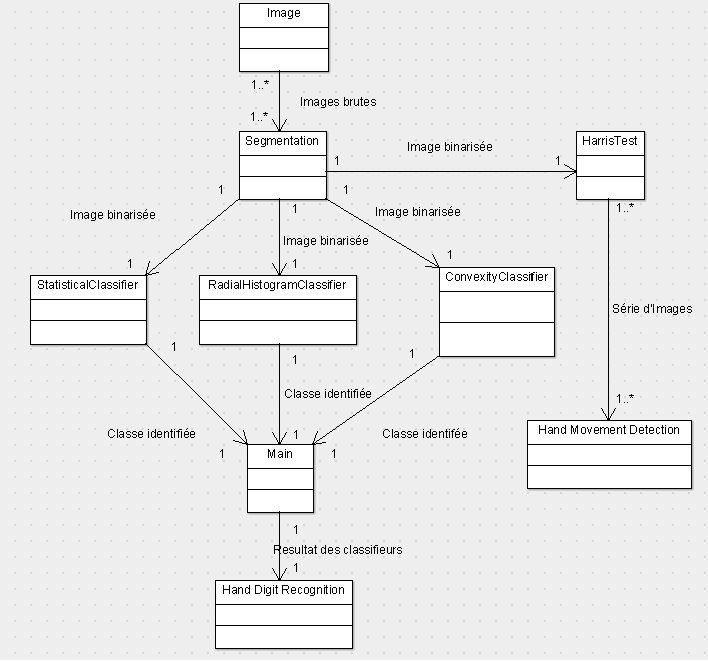
\includegraphics[scale=0.6]{Diagramme_classes.png}}
\caption{Diagramme de classe simplifié du programme}
\label{fig:diagrammeClasses}
\end{figure}